\label{ch:groups}
\newcommand{\ev}{\mathrm{ev}}
\section{desiderata}\footnote{the exercises/definitions of this section should go in a previous chapter}
The following definitions/exercises/notations/etc is used, but should probably be elsewhere.

\subsection{Request wrt notation}
\label{sec:requestnotation}

If $f:A\to B$ and $(a,p):f^{-1}(b)$ (for $a:A$, $b:B$ and $p:f(a)=b$), then the function
$$\mathrm{ad}_p\ap f:(a=a)\to(b=b)$$
needs a simpler name.  I have occasionally sinned and called it $f^=$ (with $p$ implicit).  

\subsection{Move to ``More on Natural numbers''}
\label{sec:moonN}
\begin{lemma}\label{lem:Nwellordered}
  As an ordered set, the natural numbers are well ordered: any nonempty decidable subset of $\NN$ has a minimum.\footnote{move to around \cref{def:Niswellordered} (the statement I want to refer to is somewhat simpler than what is stated there).  Btw. Pigeonhole is in one word}
\end{lemma}
\begin{corollary}
  \label{cor:arch}
  If $m,n:\NN$ and $m$ is positive (\ie $0<m$), then there is a $k:\NN$ with 
$$mk\leq n<m(k+1).$$
\end{corollary}
\begin{proof}
  Recall from \cref{lem:dec-eq+order-N} that the order relation on $\NN$ is decidable.
  Note that $$n=1\cdot n\leq m\cdot n<m\cdot n+m=m(n+1)$$ and so the decidable set of $k:\NN$ such that $n<m(k+1)$ is nonempty. By \cref{lem:Nwellordered} there is a minimal $k$ with this property.  If $k=0$, then $mk=m\cdot 0=0\leq n$, and if $k=k'+1$  is positive, then $mk=m(k'+1)\leq n$ by the minimality of $k$ (c.f. \cref{xca:try-your-luck-N}).  
\end{proof}



\subsection{Type families}
\label{sec:typefam}

This is just a placeholder for the following result and variants (Marc and Ulrik will place it somewhere)
\begin{lemma}
\label{lem:typefamiliesandfibrations}
  Lat $A$ be a type.  Then
$$\mathrm{preim}:\sum_{B:\UU}(B\to A)\quad\to\quad (A\to\UU) 
$$ 
given by $\mathrm{preim}(B,f)(a)=f^{-1}(a)$ is an equivalence.\footnote{in some higher universe}
An inverse equivalence is given by sending $P:A\to\UU$ to $(\sum_{a:A}P(a), \mathrm{pr_1})$.\footnote{extend to families in other settings like sets or propositions or ...}
\end{lemma}


\subsection{Connected types}
\label{sec:connectedtypes}
Recall the definition of a contractible type.  A type is connected essentially by the same definition, with the only difference that we do not have control over a contraction, merely that each point is individually equal to some center.
\begin{definition}\label{def:connected}
A type $A$ is \emph{connected} if there is an $a:A$ such that for all $b:B$ the proposition $||a=b||$ is true.  
\end{definition}
Note that under this definition, the empty type $\bn{0} $ is not connected, and neither is $\bn{n} $ if $n>1$. However, $\bn{1} $ is connected.

Another way of saying that a type $A$ is connected is to say that the truth-value of a proposition depending on $A$ is constant, a fact which is formalized as follows.
\footnote{this proof is classical.  Do you object?.   Ulrik \emph{did} object.  
The only place where I can remember having actually planned to use  this is in \cref{lem:circleisconnected} to show that $S^1$ is connected.  However, that can be replaced by dropping the simplification at the beginning of  \cref{lem:S1groupoid} and use that the $f$ in the proof actually is an equivalence without this. 

\begin{lemma}
  \label{lem:classicalconnected}
  A type $A$ is connected if and only if the function 
$$c:\bn{2} \to(A\to\bn{2} )$$ defined by $c(x)(a)=x$ for $x:\bn{2} $ and $a:A$ 
%to the constant function with value $x$ 
is an equivalence. 
%$||A||%\sum{a,b:A}||a=b||=\bn{1} $.  
\end{lemma}
  \begin{proof}    
    Assume $A$ is connected.  Let $a:A$ be so that for every $b:A$, then $||a=_Ab||$ is true.  If $f:A\to\bn{2} $, then for every $b:A$ we get that $||f(a)=f(b)||$, but since $\bn{2} $ is a set, we get that $f(a)=f(b)$.  Hence, any function $f$ is constant and so $c$ is an equivalence.

Conversely, assume that $c$ is an equivalence.  Then $A$ is nonempty.  Let $a:A$ and let $f:A\to \bn{2} =\bool$ be defined by $f(b)\defequi||a=b||$.  Since $c$ is an equivalence and $f(a)$ is true, we get that $f(b)$ is true for all $b$.   
  \end{proof}
}

 As a matter of fact, if $A$ has an element $a$, then $A$ is connected if and only if for all $b:A$ the identity type $a=_Ab$ is inhabited, essentially because if $f\colon A\to\bn{2} $ an equality $a=_Ab$ forces $f(a)=_{\bn{2} }f(b)$.  So, a connected type is one that can't be ``torn apart''.  
\begin{definition}
    If $A$ is a type and $a:A$, then the \emph{component of $a$ in $A$} is the type
$$A_{(a)}\defequi \sum_{b:A}||b=a||.$$
\end{definition}
\begin{xca}
  Prove that the component of $a$ in $A$ is connected.  

 [\footnote{This tries to say that, nonfunctorially, a space is the disjoint union of its components.  Don't think we need it so it can propably be thrown away.}Assuming the appropriate form of axiom of choice \footnote{someone insert our choice}, prove that the path components define a family $A\to\UU$ factoring as $A\to||A||$ making sense of the equation ``$||A=\sum_{[a]:||A||}A_{[a]}||$''.]
\end{xca}
\begin{xca}\label{xca:essentiallysmall} \footnote{Some version of this will probably be needed.  It won't be used in any cases where functoriality is needed.}
  Let $\UU\subseteq\UU_1$ be universes and let $A:\UU_1$ so that $||A||$ is in $\UU$ and for all $a,b:A$ we have that $(a=_Ab):\UU$.  Then $A$ is \emph{essentially small}, \ie there is an equivalence (in $\UU_1$) to a type in $\UU$.  

Prove that if $n:\NN$ then the type $\fin_n$ of sets of cardinality $n$  (c.f.~\cref{def:finiteset}) is essentially small, and more generally that if $S$ is a set, then the component $\Set_{(S)}$ is essentially small.  
\end{xca}
\cref{xca:essentiallysmall} has the consequence that in many cases types and essentially small types can be used interchangeably.  Where this may clutter the notation we will gloss over this distinction.

\subsection{Pointed types}
\label{sec:poitedtypes}
\begin{definition}\label{def:pointedtypes}
  A \emph{pointed type} is a pair $(A,a)$ where $A$ is a type and $a$ is an element of $A$, so that the (large) \emph{type of pointed types} is
$$\UU_*=\sum_{A:\UU}A.$$
Given a type $A$ we let $A_+$ be the pointed type you get by adding an element: $A_+\defequi(A\coprod\true,\inr{\triv})$, and given a pointed type $B=(A,a)$, the \emph{underlying type} is $B_\div\defequi A$, and the \emph{base point} is $\pt_B=a$ (so that $B\oldequiv (B_\div,\pt_B)$).  

If $(A,a)$ and $(A',a')$ are pointed types,  \emph{pointed map} from  $(A,a)$ to $(A',a')$ is a map $f:A\to A'$ together with an element $p:f(a)=a'$.  In other words, the \emph{type of pointed maps} from a pointed type $B$ to another $B'$ is
$$(B\to_*B')=\sum_{f:B_\div\to B'{}_\div}f(\pt_B)=\pt_{B'}.$$
\end{definition}
\begin{remark}
  It is customary to be sloppy regarding the distinction between $B$ and $B_\div$  when there is no chance for confusion; for instance, if $B$ is a pointed type ``$b:B$'' is taken to mean $b:B_\div$, and a type family $B_\div\to\UU$ will often be referred to as ``$B\to\UU$''.
\end{remark}

\begin{xca}\label{xca:plusforgetadjoint}
  If $A$ is a type and $B$ is a pointed type, prove that $A\to B_\div$ is equivalent to $A_+\to_*B$.
\end{xca}
\begin{xca}\label{xca:freemaps}
  Let $A$ be a pointed type and $B$ a type.  Show that the projection  
$$\mathrm{pr}_2:\sum_{b:B}(A\to_*(B,b))\to (A_\div\to B)$$
given by $\mathrm{pr}_2(b,f,p)=f$ (for $b:B$, $f:A_\div\to B$ and $p:f(\pt_A)=b$) is an equivalence.
Hint: note that 
$$\sum_{b:B}(A\to_*(B,b))\oldequiv \sum_{b:B}\sum_{f:A_\div\to B}f(\pt_A)=b$$ is equivalent to $\sum_{f:A_\div\to B}\sum_{b:B}f(\pt_A)=b$.
%Hint: show that the fiber $\sum_{b:B}\sum_{g:A_\div\to B}\sum_{p:g(\pt_A)=b}f=g$ over $f:A_\div\to B$ is equivalent to $\sum_{b:B}f(\pt_A)=b$ which is contractible.
\end{xca}



\subsection{Coverings}
\label{sec:covering}
% {\color{red}Trying Alternative version:
% \begin{definition}
%   \label{def:covering}
%   Let $B$ be a type.  A \emph{covering of $B$} is a family of sets $F:B\to\Set$.
%   A function $f:A\to B$ between two types is a \emph{covering} if for all $b:B$. We say that the covering is \emph{decidable} if for all $b:B$ the set $F(b)$ is decidable.
%   Given a covering $F:B\to\Set$, the identity type $F=_{B\to\Set B}F$ is called the type of \emph{deck transformations}.
% \end{definition}

% Traditionally, a covering is a function $f:A\to B$ so that for each $b:B$ the preimage $f^{-1}(b)$ is a set.  We see that if $F:B\to\Set$ is a covering in our sense, then the first projection $\mathrm{pr}_1:\sum_{b:B}F(b)\to B$ is a covering in the traditional sense. 
%   }


\begin{definition}
  \label{def:covering}
  A function $f:A\to B$ between two types is a \emph{covering} if for all $b:B$ the preimage $f^{-1}(b)$ is a  set.  We say that the covering is \emph{decidable} if the preimages are decidable sets.
\end{definition}

So, in particular, equivalences are coverings. Figure~\ref{fig:covering} displays a non-trivial covering of the circle.
\begin{figure}
  \centering
  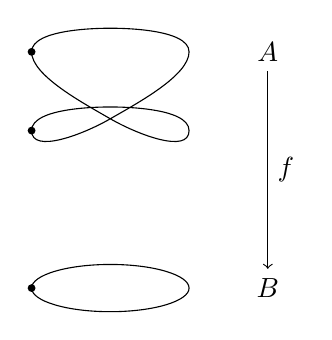
\begin{tikzpicture}
    \node (A) at (2,1) {$A$};
    \node (B) at (2,-2) {$B$};
    \draw[->] (A) -- node[auto] {$f$} (B);
    \draw (0,-2) ellipse (1 and .3);
    \draw (-1,0)
    .. controls ++( 90:-.3) and ++(210: .4) .. (0,0.15)
    .. controls ++(210:-.4) and ++(270: .3) .. (1,1)
    .. controls ++(270:-.3) and ++(  0: .1) .. (0,1.3)
    .. controls ++(  0:-.1) and ++( 90: .3) .. (-1,1)
    .. controls ++( 90:-.3) and ++(150: .4) .. (0,0.15)
    .. controls ++(150:-.4) and ++(270: .3) .. (1,0)
    .. controls ++(270:-.3) and ++(  0: .1) .. (0,0.3)
    .. controls ++(  0:-.1) and ++( 90: .3) .. (-1,0);
    \node[fill,circle,inner sep=1pt] at (-1,-2) {};
    \node[fill,circle,inner sep=1pt] at (-1,0) {};
    \node[fill,circle,inner sep=1pt] at (-1,1) {};
  \end{tikzpicture}
  \caption{A covering of the circle}
  \label{fig:covering}
\end{figure}


To sum up with a formula, 
given a type $B$, the type of coverings of $B$ is
$$\sum_{A:\UU}\sum_{f:A\to B}\prod_{b:B}\isset(f^{-1}(b)),$$ 
or equivalently, to the type of type families
$$B\to\Set.$$
Hence, an equality of coverings $(A,f,!)=(A',f',!)$ is equivalent to 
$$\sum_{p_A:A=_{\UU}A'}(f'p_A=_{A\to B}f).$$
\begin{definition}
  Let $f:A\to B$ be a covering.  A symmetry $(A,f,!)=(A,f,!)$ is called a \emph{deck transformation}.
\end{definition}
%specified by a pair $(p_A,p_f)$ with consisting of a $p_A:A=_{\UU}A'$, a $p_f:f'p_A=_{A\to B}f$.

\subsection{Equivalences and coverings of connected types}
\label{sec:eqconntypes}((to be moved AFTER connected types, coverings and injections))

\begin{lemma}
  \label{lem:eqandcovofconntypes}
  Let $X$ and $Y$ be types, $x_0,x_1:X$, let $f:X\to Y$ be a function and let $q:f(x_0)=_Yf(x_1)$. Let 
    $$%f^=_{x_0,x_1}
\ap f:(x_0=_Xx_1)\to (f(x_0)=_Yf(x_1))$$
be the function of \cref{def:apd} induced by $f$.  Then the following types are equivalent
  \begin{enumerate}
  \item the preimage of $q$ of $\ap f$,  
  \item $(x_0,\refl{y_0})=_{f^{-1}(y_0)}(x_1,q)$ and
  \item $\sum_{p:x_0=x_1}q=\ap f(p)$.
  \end{enumerate}
If in addition $X$ and $Y$ are connected, then
\begin{enumerate}
\item $f$ is an equivalence if and only $\ap f%f^=_{x_0,x_1}
$ is an equivalence and
\item $f$ is a covering if and only if  $\ap f%^=_{x_0,x_1}
$ is an injection.
\end{enumerate}

\end{lemma}
\begin{proof}
  Steal and adapt the one below (and then delete the below).
\end{proof}

\begin{lemma}\label{lem:eqofconntypes}\footnote{
%The argument for a general group and the torsors over its abstract group is VERY similar.  
Essentially it is our version of ``a group homomorphism is an isomorphism iff it is a bijection'': proofread}
  Let $X$ and $Y$ be connected types, $x_0:X$ and let $f:X\to Y$ be a function.  Then $f$ is an equivalence if and only if the induced function from $x_0=x_0$ to $f(x_0)=f(x_0)$ is.\footnote{note to self: try to be consistent in writing equalities with right variance (as I hope I have managed to do here)}
\end{lemma}
\begin{proof}
  If $f$ is an equivalence, it follows automatically that the function of identity types is, so we concentrate on the other implication and assume the induced function from $x_0=x_0$ to $f(x_0)=f(x_0)$ is an equivalence.  We want to show that all fibers of $f$ are contractible, but since $Y$ is connected it is enough to consider the fiber $f^{-1}(y_0)\defequi\sum_{x:X}y_0=f(x)$ over $y_0\defequi f(x_0)$.  

Consider the induced map $Pf$ from $\sum_{x:X}x_0=x$ to $\sum_{y:Y}y_0=y$.  Its fiber over $(y_0,\refl{y_0})$ is 
$$(Pf)^{-1}(y_0,\refl{y_0})\oldequiv\sum_{x:X}\sum_{p:x_0=x}\sum_{q:y_0=f(x)}q=f(p),$$ and is contractible since it is the fiber of a map of contractible types.  We see that the projection $(Pf)^{-1}(y_0,\refl{y_0})\to f^{-1}(y_0)$ is an equivalence once we notice that the fiber over $(x_1,q:y_0=f(x_1)) $ is equivalent to the fiber $\sum_{p:x_0=x_1}q=f(p)$ over $q$ of the induced function $x_0=x_1$ to $y_0=f(x_1)$.
\end{proof}
\begin{lemma}
  Let $X$ and $Y$ be connected types, $x_0:X$ and let $f:X\to Y$ be a function.  Then $f$ is a covering if and only if the induced function from $x_0=x_0$ to $f(x_0)=f(x_0)$ is an injection.\footnote{embedding/injection...}
\end{lemma}



\subsection{Negative numbers}
\label{sec:negativenumbers}

 \begin{example}\label{ex:orbitofanelement}
   Given a pointed type $a:A$ and an element $g: a=_Aa$ we can iterate $g$ any number of times to get a (potentially) new element in $a=_Aa$. More precisely, for $n:\NN$ we define $g^n:a=_Aa$ by declaring that $g^0=\refl a$ and $g^{n+1}=\trans{}_{a,a,a}(g^n)(g)$.  We can also give meaning to $g^{-n}$ by setting it equal to $(\symm{}_{a,a}(g)^n$ (prove that $g^{-n}=(g^n)^{-1}$ and that $g^a\cdot g^b=g^{a+b}$).  \footnote{come back to this example in conjuction with $S^1$, show how to get it as an abstract group, connect it to orbits.}

Note that we can have that $g^n=g^m$ even if $m$ and $n$ are different.  For instance, in $\Sigma_2=\aut_{\fin_2}(\bn{2} )$, consider the element $p:\bn{2} =\bn{2} $ defined by $p(1)=2$ and $p(2)=1$.  Then $p^2(1)=p(2)=1$ and $p^2(2)=p(1)=2$, so that $p^2=e=p^0$.
   \end{example}
This example tells us that if we want to start counting symmetries we should extend our type $\NN$ of natural numbers to include negatives.  Rather than ``adjoining negatives'' we do as we do when we define the rationals: heuristically, an integer is the set of pairs $(m,n)$ of natural numbers, subject to the relation that $(m,n)=(m',n')$ if $m+n'=m'+n$.\footnote{picture}.  If $m\geq n$, then $(m,n)=(m-n,0)$ and if $m\leq n$, then $(m,n)=(0,n-m)$.  We include the natural numbers as classes of the form $(m,0)$ and call the ones of the form $(0,n)$ ``negative numbers''.  The formal definition is as follows.
\begin{definition}
  \label{def:zet}\footnote{To the one who ports: I \emph{would} have preferred to define $\zet$ as a set quotient of $\NN\times\NN$, but I hoped we could avoid the book discussion (257).  A price is paid when defining the successor.  Given the disclaimer following the formal definition, it is safe to change the definition if you like}
  The \emph{set of integers} is the set
$$\zet\defequi \sum_{(m,n):\NN\times\NN}(r(m,n)=_{\NN\times\NN}(m,n)),$$
where $r:\NN\times\NN\to\NN\times\NN$ is given by
$$r(m,n)\defequi
\begin{cases}
  (m-n,0)&\text{if $m\geq n$}\\
  (0,n-m)&\text{otherwise.}
\end{cases}
$$
We define the \emph{standard inclusion} 
$$i:\NN\to\zet$$ by $i(m)=((m,0)\refl {(m,0)})$ (makes sense since $r(m,0)\defequi(m,0)$), the \emph{negative inclusion} $-:\NN\to\zet$ by $-n=((0,n),\refl{(0,n)})$ and the quotient $q:\NN\times\NN\to\zet$ by $q(m,n)=(r(m,n),\refl{r(m,n)})$ (makes sense since $r(r(m,n))\oldequiv r(m,n)$).  

The successor $s:\zet=\zet$ is defined through univalence from $S\colon\NN\times\NN\to\NN\times\NN$ with $S(i(n))=i(S(n))$  and $S(-(Sn))=-n$ for $n:\NN$ (check that $S$ is an equivalence: ``any integer is the successor of exactly one integer'').
\end{definition}

Not wishing to mystify things more than necessary, we will refer to $i(n):\zet$ for $n:\NN$ as ``$n:\zet$'', so that any element of $\zet$ is ``plus or minus a natural number'', dividing the non-zero integers into the positive and negative integers.  We extend the order relation by saying that positive integers are greater than negative integes and by saying that $-m\leq -n$ if $n\leq m$ for $m,n:\NN$.

% \subsubsection{Equivalences}
% \label{sec:equivalences}
% Two types are equivalent if you can freely translate back and forth between them: 
% \begin{definition}
%   Let $A$ and $B$ be types.  The type of \emph{equivalences} from $A$ to $B$ is
% $$\Eq(A,B)\defequi\sum_{f: A\to B}\left(\sum_{g:B\to A}\prod_{a:A}g(f(a))=a\right)\times\left(\sum_{h:B\to A}\prod_{b:B}f(h(b))=b\right).
% $$
% \end{definition}
% \begin{remark}
%   You recognize the spirit of ``inverse function'' in the definition of equivalences: an equivalence is a function $f:A\to B$ which has a $g:B\to A$ so that for all $a:A$ we have $g(f(a))=a$ and also an $h:B\to A$ so that for all $b:B$ we have that $f(h(b))=b$.  We will see in Lemma~\ref{lem:leftinvisrightinv} that this forces $g$ and $h$ to be equal, but it is technically convenient not to insist on this in the definition itself.  We refer to $g$ as a \emph{left inverse} of $f$ and $h$ as a \emph{right inverse} of $f$.
% \end{remark}


% \begin{lemma}
%   Given $f\colon A\to B$, the type of left inverses of $f$, 
% $$\sum_{g:B\to A}\prod_{a:A}g(f(a))=a,$$ is a proposition.  Consequently, the projection $\Eq(A,B)\to (A\to B)$ is a monomorphism.
% \end{lemma}
% \begin{proof}
%   ((write)) 4.2.9
% \end{proof}
% \begin{remark}
%   In view of this result, we will say that $f:A\to B$ \emph{is an equivalence from $A$ to $B$} if it is the projection of an equivalence from $A$ to $B$.  Occasionally the following alternative notation is more convenient:
% $$(A\simeq B)\defequi\Eq(A,B),$$
% and ocasionally we'll be sloppy and write $f:A\simeq B$ instead of the actual tuple $(f,(g,p),(h,q))$, hiding the (unique) choice proving that we actually are talking about an equivalence. 
% \end{remark}

% \begin{lemma}\label{lem:leftinvisrightinv}
%   The left and right inverses of an equivalence are equal.\footnote{check compatibility of notation and agree whether the carefree language is ok}
% \end{lemma}
% \begin{proof}
%   Let $(f,(g,p),(h,q)):\Eq(A,B)$. Then, for all $b:B$ we have $g(q_b):g(f(h(b))=g(b)$,  and $p_{h(b)}:g(f(h(b)))=h(b)$, and so, using symmetry and transitivity of the identity type, we have that $g(b)=h(b)$. 
% \end{proof}
% \begin{example}
%   If $A$ is a type, then the identity map $\id_A:A\to A$ (given by $\id_A(a)=a$) is an equivalence: it is its own (left and right) inverse, with $\refl a:\id_A(\id_A(a))=a$ as witness(es).  
% \end{example}


% \begin{remark}
%   Inspired by sets, one can think of another possible definition of equivalence: namely a function $f:A\to B$ is a bijection if it is one-to-one and onto.  Spelling this out in detail, it means that for evey $b:B$ there is \emph{exactly one} $a:A$ such that $f(a)=b$.  The inverse of $f$ is then constructed by sending $b:B$ to the unique $a:A$ with $f(a)=b$.  The set of $a:A$ with $f(a)=b$ is called the ``preimage'' or ``fiber'' $f^{-1}(b)$ over $b$, and the condition then reads that ``for every $b:B$ the fiber over $b$ contains exactly one element''.  This works in our setting as well.  
% \end{remark}
% We must first transcribe these notions to our setting.
% \begin{definition}
%   The \emph{fiber} of a function $f:A\to B$ and $b:B$ over an element $b:B$ is the type
% $$f^{-1}(b)=\sum_{a:A}f(a)=b.$$
% The type of \emph{contractions} of a type $A$ is
% $$\iscontr(A)\defequi\sum_{a:A}\prod_{x:A}a=x.$$
% \end{definition}
% Note that an element in $\iscontr(A)$ consists of a point $a:A$ and for every $x:A$ a $p_x:a=x$, that is, a proof of the assertion that all elements of $A$ are equal to $a$.  

% If $f:A\to B$ is a function of types, we say that $f$ i a \emph{weak equivalence} if for every $b:B$ there is an $a:A$ such that for all $x:A$ with $f(x)=b$ we have a $p_x:a=x$.  More precisely:


% \begin{definition}
%   If $A$ and $B$ are types, the type of \emph{weak equivalences} from $A$ to $B$ is
% $$\wEq(A,B)=\sum_{f:A\to B}\prod_{b:B}\sum_{a:A}\prod_{x:A}
% $$
% \end{definition}




\section{The circle}
\label{sec:sec:circle}
[this is potentially going to be a separate chapter.  if so it is going to have an introduction (I can't but help to think of grand suggestions about symmetries) and so on.  The following is a list of place holders for some mathematics we're going to want to include]

\begin{definition}
  \label{def:circle}
The circle $S^1\colon\UU$ ((write and point it at $\base$.  The loop is going to be called $\Sloop$))
\end{definition}
The following Lemma displays the perhaps most fundamental property of the circle: a function from the circle picks out an element and a symmetry of that element:
\begin{lemma}\label{lem:freeloopspace}
  If $A$ is a type, the function in $$(S^1\to A)\to \sum_{a:A}(a=_Aa)$$
given by sending $g$ to $(g(\base),g(\Sloop))$ is an equivalence.  In particular, if $a:A$, the function in $((S^1,\base)\to_* (A,a))\to (a=_Aa)$ given by sending $g:S^1\to A$ to $g(\Sloop)$ is an equivalence. 
\end{lemma}
\begin{proof}
  ((write)) 6.2.9
\end{proof}
\begin{remark}
  A function $\gamma:S^1\to A$ is often referred to as a \emph{loop}: the picture being that $\gamma$ throws $\Sloop:\base=\base$ as a lasso in the type $A$.

  Under univalence, so that $a=_Aa$ is identified with the pointed functions from the circle, this allows for a very graphic interpretation of the symmetries in $a=_Aa$: they are all in the image of a function $g$ from the circle: they are loops in the type $A$ starting and ending at $a$!
\end{remark}


\footnote{The current proof of the circle being connected uses \cref{lem:classicalconnected}.  This must be fixed, eg as suggested in the footnote where \cref{lem:classicalconnected} has been put.  Can also use the version where $\bn 2$ is replaced by an arbitrary finite set}
\begin{lemma}\label{lem:circleisconnected}
  The circle is connected.
\end{lemma}
\begin{proof}
  We need to prove that the function $\bn{2} \to(S^1\to\bn{2} )$ of \cref{def:connected} is an equivalence.  In view of \cref{lem:freeloopspace} it is enough to show that the composite
$$\bn{2} \to \sum_{a:\bn{2} }(a=_{\bn{2} }a)$$
sending $a:\bn{2} $ to $(a,\refl a)$ is an equivalence.  Composing further with the first  projection $\mathrm{pr}_1:\sum_{a:\bn{2} }(a=_{\bn{2} }a)\to\bn{2}$ we get the identity on $\bn 2$, so it suffices to show that $\mathrm{pr}_1$ is an equivalence.  This is true since the fibers $\mathrm{pr}_1^{-1}(a)\simeq (a=_{\bn{2} }a)$ are contractible.
\end{proof}


\begin{lemma}\label{lem:S1groupoid}
  The circle $S^1$ is a groupoid and $\Sloop^-:\zet\to(\base=_{S^1}\base)$ sending $n$ to $\Sloop^n$ is an equivalence.
\end{lemma}
\begin{proof}
  Since the circle is connected, for any $z,w:S^1$ the type $z=_{S^1}w$ is equivalent to $z=_{S^1}\base$, so it is enough to prove the last statement.  Define two type families 
$$P,R:S^1\to\UU$$ (actually, both families have values in sets).  The first is the family defined by $P(z)\defequi(z=\base)$ for $z:S^1$ and the second is defined by the induction priciple for the circle by  % $E(\Sloop)(p)=\trans{}_{z,\base,\base}(p)(\Sloop):(z=\base)$
$R(\base)=\zet$ and $R(\Sloop)=\ua(S):(\zet=\zet)$, where $S$ is the successor function.\footnote{must define.  Shall $\ua$ be visible?}%8.1
Transport defines a function $f:\prod_{z:S^1}(P(z)\to R(z))$, with $f(z)(p)\defequi\trp_{R,p}0$.
((finish!!! e.g. as in the book))
\end{proof}
\begin{remark}
  Through \cref{lem:freeloopspace} we can get a different perspective on the circle which highlights it as a type classifying very simple symmetries.
By \cref{lem:freeloopspace} (moving up one universe), a type family $S^1\to\UU$ is uniquely given by a type $X:\UU$ together with a $p:X=_\UU X$, with no further requirements on $p$.  We have seen one example in \cref{def:zet}, namely the one given by the set $\zet$ of integers together with the element $s:\zet=\zet$ given by the successor.  

The importance of this example will become apparent when we eventually explain that \emph{the circle is equivalent to the component $C$ of $\sum_{X:\UU}(X=_{\UU}X)$ containing $(\zet,s)$}. 

Heading towards this goal, we investigate this component a bit further.  Recall from \cref{sec:identity-types} that, in general, if given elements $x,y,z$ in a type $A$, and two identities $f:x=y$ and $g:y=z$, then transport gives rise to the ``composite identity'' $gf:x=z$ (aka $g\circ f$).    Now, if $(X,f):\sum_{X:\UU}(X=_{\UU}X)$, then an element in the identity type $(\zet,s)=(X,f)$ consists of a $p:\zet=X$ and a proof that the succesor $s:\zet=\zet$  is transported along $p$ to $f:X=X$, that is, an element in $psp^{-1}=_{X=X}f$.  Now, by transport, $psp^{-1}=_{X=X}f$ is equivalent to $fp=_{\zet=X}ps$, and so the identity type $(\zet,s)=(X,f)$ is equivalent to
$$\sum_{p:\zet=X}fp=_{\zet=X}ps.$$ % the equation $fp=ps$ comes from the fact that equality in the identity type means that the transport of $s$ along $p$ is equal to $f$, in other words we have an element in $p^{-1}sp=_{X=X}f$ (which we have translated for convenience to an element in $fp=_{\zet=X}ps$).
Since $\zet$ is a set, this identity type is a proposition and so our component $C$ is a connected groupoid.  

In particular, the type of symmetries $(\zet,s)=_C(\zet,s)$ is equivalent to $\sum_{p:\zet=\zet}sp=ps$.  

This discussion tells us that the following definition makes sense:

\begin{definition}\label{def:S1toC}
  Let $C$ be the component of $\sum_{X:\UU}(X=_{\UU}X)$ containing $(\zet,s)$.
  Let $$c:S^1\to C$$ be defined by $c(\base)\defequi (\zet,s)$ and $c(\Sloop):((\zet,s)=_C(\zet,s))$\footnote{atrictly speaking, this $c$ is $\ap c$ -- I have decided not to distinguish between them; ok?} be given by the successor $s:\zet=\zet$ (and $\refl{}:ss=ss$)
\end{definition}

We are going to prove that $c$ is an equivalence.  This is greatly simplified by the fact that we already know that both $S^1$ and $C$ are connected groupoids, since then \cref{lem:eqofconntypes} says that it is enough to show that $c$ induces an equivalence of symmetries.\footnote{of course, the proof of \cref{lem:S1groupoid} \emph{could} attack $c$ directly, but that would compound the technicalities already present there: at present I prefer splitting it up like this.  I am open for letting the proof of \cref{lem:S1groupoid} be postponed till the end of a chapter, so as not to disrupt the flow of ideas}

\begin{lemma}
  \label{lem:IdCisZet}
  Any element in $(\zet,s)=_C(\zet,s)$ is of the form $(s^k,!)$ for some unique $k:\zet$.  In other words,
  the function 
$$\ev_0:((\zet,s)=_C(\zet,s))\to \zet$$ given by $\ev_0(p)=p(0)$ is an equivalence.
\end{lemma}
\begin{proof}
  Given $(p,!):(\zet,s)=_C(\zet,s)$ we must determine $p:\zet=_{\Set}\zet$, which by univalence amounts to giving all the values $p(n)$ for $n:\zet$.  However, since $sp=ps$ we get that $p(n+1)=p(n)+1$ and so induction on $n$ (induction for positive and negative $n$ separately) gives that $p(n)=n+p(0)$.  Hence, $p=s^{p(0)}$ (uniquely since $\zet:\Set$).
\end{proof}


\begin{theorem}\label{thm:S1bysymmetries}
  The function $c:S^1\to C$ is an equivalence.
\end{theorem}
\begin{proof}
  In view of \cref{lem:eqofconntypes} we only need to show that the induced function of symmetries $c:(\base=_{S^1}\base)\to((\zet,s)=_C(\zet,s))$ is an equivalence.\footnote{ ((can we call equivalences between sets bijections?)).}  

The function $\Sloop^-:\zet\to (\base=_{S^1}\base)$ sending $n:\zet$ to $\Sloop^n$ is an equivalence by  \cref{lem:S1groupoid} and the function  $\ev_0:((\zet,s)=_C(\zet,s))\to \zet$ given by $\ev_0(p)=p(0)$ is an equivalence by \cref{lem:IdCisZet}.  Tracing through the composite function $\ev_0c\Sloop^-:\zet\to\zet$ we see that $\ev_0c\Sloop^n=\ev_0s^n=n$, (\ie $\ev_0c\Sloop^-=\id_\zet$) giving that $c$ is an equivalence. 
% The composition with the functions $\Sloop^-:\zet\to (\base=_{S^1}\base)$ sending $n:\zet$ to $\Sloop^n$ and $\ev_0:((\zet,s)=_C(zet,s))\to \zet$ of \cref{lem:IdCisZet} given by $\ev_0(p)=p(0)$ gives us a function $w:\zet\to\zet$ with $w(n)=s^n(0)$.  From \cref{lem:S1groupoid} we know that $\Sloop^-$ is an equivalence, so we only need to show that $w$ is an equivalence
\footnote{I may have used 2-out-of-3 before, we probably need to include it somewhere, though by univalence it hardly seems necessary}% .  If $p:\zet=\zet$ with $!:sp=ps$, we get by induction on $n:\zet$ (induction for positive and negative $n$ separately) that $p(n)=n+p(0)$.  Hence, all the elements in the preimage $w^{-1}(p,!:sp=ps)$ are equal to $(p(0),!)$.  
\end{proof}

% Now, consider the function 
% $$f:\sum_{p:\zet=\zet}(sp=ps)\to\zet,\qquad f(p,!)=p(0).$$  If $a:\zet$, then $f^{-1}(a)$ consists of the $p:\zet=\zet$ with $sp=ps$ and $p(0)=a$ (the last two are propositions), but by induction we see that $p(n)=n+a$ for all $n:\zet$ (separate induction on positive and negative numbers).  In other words, all elements in the set $f^{-1}(a)$ are equal, and so $f$ is an equivalence


%   ((TODO))
% As an illustration of things to come in a simpler setting, we can give the torsor definition of the circle, where Marc makes the simplifying observation that (since the integers is free on one generator) this can be coded in terms of the successor and there is a priori no need to talk about the abstract group.  In short: an (abstract) $\ZZ$-set is uniquely given by a set $X$ with an identity $f: X=_{\Set}X$.  A $\ZZ$-torsor $(X,f)$ is a $\ZZ$-set (merely) equal to $(\zet,S)$ ($S$ is the successor), that, there is a $p:X=\zet$, so that $Sp=_{X=X} pf$.  This is based at (the pricipal $\ZZ$-torsor represented by) $(\zet,S)$ and $(\zet,S)=(\zet,S)$ consists of $f:\zet=\zet$ s.t. $Sf=fS$.  Such an $f$ must be given by addition by the integer $f(0)$.  This gives us an equivalence between $S^1$ and the type of (secret) $\ZZ$-torsors.  This will be trivial if we have shown that a map of connected groupoids is an equivalence if it induces an equivalence on the identity sets.
\end{remark}

\subsection{Coverings of the circle}
\label{sec:covS1}

\footnote{The below is not fully structured yet, and does contain known nonsense (basepoints, orientations etc need to be straightened out)}
From \cref{lem:eqandcovofconntypes} we know that a function $f:A\to S^1$ from a connected type $A$ is a covering if and only if for given $a_0:f^{-1}(\base)$ the induced function from $a_0=_Aa_0$ to $(f(a_0)=f(a_0))=(\base=_{S^1}\base)$ is injective; or in words, if the symmetries of $a_0$ inject into the symmetries of $\base$ (which by \cref{lem:S1groupoid} may be identified with with the set $\zet$ of integers).

So, a classification of coverings of the circle amounts to answering the question of what ``subsymmetries'' $\base$ posesses.  Using language yet to be introduced, the question would be ``what are the subgroups of the integers?''

\begin{example}
  \label{ex:listofS1covers}
  In the course of our discussion, we will see that -- under an assumption on the setup called ``LPO'' -- the following represent all the connected decidable coverings of the circle.
  \begin{enumerate}
  \item The \emph{universal} connected cover  $$c_\base:\bn 1\to S^1$$ sends the unique element of $\bn 1$ to $\base$ is a covering corresponding to the trivial symmetry of $\base$ (\ie only $\refl\base$).  
  \item If $m:\NN$ is positive, consider the \emph{degree $m$ function} $$-^m:S^1\to S^1$$ given by $-^m(\base)\defequi\base$ and $-^m(\Sloop)\defequi\Sloop^m$.  On the level of identity types and under the equivalence $\Sloop^-:\zet\simeq(\base=_{S^1}\base)$, this covering corresponds to the function $\zet\to\zet$ given by multiplication by $m$.
  \end{enumerate}
\end{example}

\begin{remark}
  \label{rem:RtoS1}
  The first case, namely the manifestation of the contractible type as a covering of the circle is important in many applications.  Classically it corresponds to the trigonometric functions sending the real number $x$ (the real numbers form a contractible space) to the point $(\cos x,\sin x)$ on the unit circle in the plane.  If you're familiar with complex numbers, you may want to say that this covering is the exponential function sending the real number $x$ to the point $e^{2\pi ix}$ on the unit circle in the complex plane.

  \label{rem:finitecoveringsofS1}
  The analogue of our degree $m$ function is the $m$th power of complex numbers restricted to the unit circle.
  ((picture!!))
\end{remark}

We will be even a bit more ambitious: what is the \emph{type} of decidable coverings of the circle?  Since the type of coverings is equivalent to $S^1\to \Set$, and the fact that if $F,F':S^1\to\Set$, then $F=_{S^1\to\Set}F$ is the type $\prod_{z:S^1}(F(z)=_{\Set}F'(z))$ (which is a set\footnote{reference}), we see that the type of decidable coverings of the circle is a groupoid.  We will pin this groupoid down by first identifying the components (of which there turns out to be one for each natural number), and then analyzing one component at a time.

 Recall the function $c:S^1\to C$ of \cref{def:S1toC}.  By \cref{thm:S1bysymmetries} we know that $c$ is an equivalence, so classifying coverings of $S^1$ is equivalent to classifying coverings of $C$.  
We simplify the notation slightly, letting $\pt_C\defequi(\zet,s):C$ (the element corresponding by \cref{def:S1toC} to $\base:S^1$), and allowing ourselves to write $s:\pt_C=_C\pt_C$ instead of the more honest $(s,!):\pt_C=_C\pt_C$ (corresponding to $\Sloop:\base=\base$).


\begin{example}
 \label{ex:listofCcovers}
  Returning to \cref{ex:listofS1covers}, it is instructive to rephraze these connected coverings in terms of $C$.
  \begin{enumerate}
  \item  The universal connected cover is still represented by the constant function
    $$c_{(\zet,s)}:\bn 1\to C$$ that sends the unique element of $\bn 1$ to $(\zet,s):C$.
  \item Assume that $m:\NN$ is positive.  If $X$ is a set and $f:X\to X$ we define the \emph{ $m$th root}
$$\sqrt[m]f:\bn m\times X\to\bn m\times X$$ by setting 
$$\sqrt[m]f(i,x)=
\begin{cases}
  (i+1,x)& \text{for $i<m-1$ and}\\(0,f(x))& \text{for $i=m-1$}.\footnote{this indexing uses the incarnation $\bn m=\{0,1,\dots m-1\}$ and not $\{1,\dots,m\}$: if this is a problem we should change $\bn m$ since the indexing chosen is very convenient later.}
\end{cases}$$ 
Only one $m$th of the time does $\sqrt[m]f$ use $f$ on $X$ (the rest of the time it increases the element in $\bn m$).  This is illustrated in \cref{fig:root} with the shift by $f$ being vertical and the movement along $\bn m$ going around a circle.  
\begin{figure}
  \centering
  \begin{tikzpicture}
    \node (A) at (4,1) {\quad$\sqrt[m]f:\bn m\times X\to\bn m\times X$};
    \foreach \y in {0,1,2}
    { \begin{scope}[shift={(0,\y)}]
        \foreach \x in {0,...,4}
        { \node[fill,circle,inner sep=1pt] at (180+72*\x:1 and .3) {}; }
        \foreach \x in {0,...,3}
        { \draw[-stealth] (180+72*\x:1 and .3) arc(180+72*\x:252+72*\x:1 and .3); }
      \end{scope} }
    \foreach \y in {1,2}
    { \begin{scope}[shift={(0,\y)}]
        \draw[-stealth] (108:1 and .3)
        .. controls ++( 5:-.3) and ++(80:.2) .. (-.7,-.4)
        .. controls ++(80:-.2) and ++(90:.2) .. (-1,-1);
      \end{scope} }
    \draw[-stealth] (108:1 and .3)
    .. controls ++( 5:-.3) and ++(80:.2) .. (-.7,-.4);
    \node (dz) at (-.7,-.7) {\footnotesize$\vdots$};
    \begin{scope}[shift={(0,3)}]
      \draw[-stealth] (-.7,-.4)
      .. controls ++(80:-.2) and ++(90:.2) .. (-1,-1);
      \node (da) at (-.7,0) {\footnotesize$\vdots$};
    \end{scope}
    \draw [decorate,decoration={brace,amplitude=10pt}]
    (-1.1,-.8) -- (-1.1,2.8) node [black,midway,xshift=-20pt] {\footnotesize $X$};
    \draw [decorate,decoration={brace,amplitude=10pt}]
    (1,-1) -- (-1,-1) node [black,midway,yshift=-15pt] {\footnotesize $\bn{m}$};
  \end{tikzpicture}
  \caption{The $m$'th root of an endomorphism}
  \label{fig:root}
\end{figure}
Indeed, iterating $\sqrt[m]f$ we get $(\sqrt[m]f)^m(i,x)=(i,f(x))$; hence the term ``$m$th root'' is apt.

If $f$ is an equivalence, then so is $\sqrt[m]f$:
\begin{enumerate}
\item on one hand $(\sqrt[m]f)(j,y)$ is equal to $(0,x)$ if and only if $j=0$ and $f(y)=x$, so  $(\sqrt[m]f)^{-1}(0,x)$ is equivalent to $f^{-1}(x)$ which is contractible if $f$ is an equivalence, and 
\item on the other, if $i:\bn m$ is not $0$, then $(\sqrt[m]f)(j,y)$ is equal to $(i,x)$ if and only $j+1=i$ and and $y=x$, and so  $(\sqrt[m]f)^{-1}(i,x)$ is equivalent to  a singleton.
\end{enumerate}


Using univalence, the $m$th root construction applies not only to equivalences, but equally well to identities $f:X=_{\Set}X$; resulting in a function 
$$-^m:\sum_{X:\Set}(X=X)\to\sum_{X:\Set}(X=X),\quad -^m((X,f))=(\bn m\times X,\sqrt[m]f).$$
We now focus on  $C$, the component of $\sum_{X:\Set}(X=X)$ containing $(\zet,s)$.
Note that the function $p:\bn m\times \zet\to\zet$ given by $p(i,n)=i+mn$ is an equivalence and that 
$$p\sqrt[m]s(i,n)=i+1+mn=sp(i,n).$$  
Consequently $(\bn m\times\zet,\sqrt[m]s):\sum_{X:\Set}X=_\UU X$ is in the component of $(\zet,s)$, \ie $(\bn m\times \zet,\sqrt[m]s):C$. % In consequence, if $(X,f):C$ (\ie, $(X,f):\sum_{X:\Set}X=_\UU X$ is in the component of $(\zet,s)$) then also $(\sqrt[m]X,\sqrt[m]f):C$, giving rise to the 
Ultimately, we have defined the
 \emph{degree $m$ function} $$-^m:C\to C,\qquad -^m((X,f))=(\bn m\times X,\sqrt[m]f).$$
% , where $$\sqrt[m]X=\bn m\times X$$ and $\sqrt[m]f(i,x)=(i+1,x)$ for $i<m-1$ and $\sqrt[m]f(m-1,x)=(1,f(x))$.  We prove that $-^m((X,f))$ is in the component of $(\zet,s)$ (which was a requirement for elements in $C$).
 % Since we know that $(X,f)$ is in the component of $(\zet,s)$ it is enough consider the element $(p,!):(\sqrt[m]{\zet},\sqrt[m]s)=(zet,s)$ explicitly given by univalence through $p((i,n))=i+mn$ ((check that it gives an equivalence)).

If $(p,!):(X,f)=_C(X',f')$, then 
$$(\id\times p,!):(\bn m\times X,\sqrt[m]f)=(\bn m\times X',\sqrt[m]f')$$ 
is given by % $(\id\times p)(i,x)=(i,p(x))$ (and by 
the fact $!:(\id\times p)\sqrt[m]f=_{\bn m\times X=\bn m\times X'}\sqrt[m]{f'}(\id\times p)$\footnote{$(i,x)$ is taken to $(i+1,px)$ if $i<m-1$ and $(m-1,x)$ is taken to either $(0,f'px)$ or $(1,pfx)$ which are equal by assumption}.  In particular, letting $p\defequi s:\zet=\zet$, we get that $(\id\times s)(i,n)=(i,sn)=(\sqrt[m]s)^m(i,n)$.

This will eventually ((forwardref)) be explained in terms of the \emph{deck transformations} of the degree $m$ covering of the circle being given by the powers of $\sqrt[m]s$ in a nonunique fashion: for any $a:\zet$, the $a$th and the $(a+m)$th power of $\sqrt[m]s$ give rise to the same deck transformation.



 Note that the equivalence $c:S^1\to C$.\footnote{comeback 190104: demonstrate that the descriptions of the coverings of the circle are the same}
  \end{enumerate}
\end{example}
\begin{xca}
  Check the implicit claims in \cref{ex:listofCcovers}.  ((perhaps best to make them explicit?))
\end{xca}

Any (other) textbook will tell you that these are all the connected coverings of the circle (precisely one for each natural number), but the procedure is unfortunately not constructive: we need a further assumption which is not generally present in our setup, namely

\begin{quote}
  {\bf The Limited Principle of Omniscience} (LPO)\index{LPO}\label{LPO}\footnote{make an environment that principles can fit in and be numbered}If given a function $P:\NN\to\bn 2$, then either $P$ is constant (we have that $\prod_{n:\NN}(P(0)=P(n))$) or there is an $n_0:\NN$ such that $P(n_0)\neq P(0)$.
\end{quote}
LPO is weaker than the law of excluded middle and we are free to assume it as an axiom -- or not.  We will be explicit about where we will use it.


Fix for the moment a connected type $A$ and a decidable covering 
$$f:A\to C$$ (c.f \cref{def:covering}) and an element $\pt_A:f^{-1}(\pt_C)$.  %Assume $(\pt_A,!):f^{-1}(\pt_C)$
%Recall the element 
%$$\pt_C\defequi(s,\refl{ss}):(\zet,s)=_C(\zet,s),$$ which by \cref{def:S1toC} corresponds to $\Sloop:\base=\base$.
By \cref{lem:eqandcovofconntypes}, the fact that $f$ is a decidable covering exactly says that the induced function of identity types
$$g\defequi\ev_0f^=:(\pt_A=_A\pt_A)\to (\pt_C=_C\pt_C)=\zet$$ is injective and decidable.\footnote{say this in a way consistent with the choices of subsets/injections/embeddings}    

Assume LPO.  We are then left with two situations (use that $g$ is injective and decidable): either $\pt_A=_A\pt_A$ is contractible or there is a $p_0:\pt_A=_A\pt_A$ with $g(p_0)$ different from $0$. 

In the former case ($\pt_A=\pt_A$ is contractible), \cref{lem:eqandcovofconntypes} together with the fact that $A$ is connected implies that $A$ itself is contractible.  

On the other hand, if $p_0:\pt_A=\pt_A$ with $g(p_0)$ different from $0$, then either $g(p_0)$ or $g(p_0^{-1})$ is a positive integer.  Hence the set $H^+$ of positive integers in the image of $g$ is nonempty, and so the fact \cref{lem:Nwellordered} that $\NN$ is well ordered implies that $H^+$ has a minimum, \ie there is a $p:\pt_A=\pt_A$ with  $g(p)=m\defequi\min H^+:H^+$.  Furthermore, if $q:\pt_A=\pt_A$ is any element with $0<g(q)$, then  by \cref{cor:arch} there is a $k:\NN$ such that $g(p)k\leq g(q)<g(p)(k+1)$, or equivalently $0\leq g(q)-g(p)k< g(p)$.  Since $g(q)-g(p)k=g(qp^{-k})$ is a nonnegative integer is in the image of $g$ and simultaneously less than the minimum positive value $g(p)$, we must conclude that $g(q)=g(p)k$.

Arguing similarly for the negative values, we reach the conclusion that the image of $g$ in $\zet$ is the subset of multiples of $g(p)=\min H^+$.  Hence, the image of $f^=:(\pt_A=\pt_A)\to(\base=_{S^1}\base)$ is uniquely given by the positive integer $\min H^+$, and is not dependent on $\pt_A$.\footnote{how to say this gently without starting to much fuss regarding commutativity?}  Furthermore, if $p_A:A=_{\UU}A'$, $f':A'\to B$ and $p_f:f'p_A=_{A\to B}f$, then tracing through the argument, we see that the positive number reached through arguing with $f':A'\to B$ remains the same, but there \emph{is} a possibility that $g(p_0)$ changes sign, so that the minimum of $H^+$ is now not attained by $g(p_0)$, but by $g(p_0^{-1})$.\footnote{maybe some HoTT guy can say this less classically.  We also want to say something about the connection to pointed coverings, conjugations etc to clear the path for later applications}

\begin{lemma}
  \label{lem:componentsofcoversofS1}
  Assume the LPO. Given a connected decidable covering of the circle,  there is a unique natural number $m$ so that the connected covering is equal to the connected covering $c^m$ of \cref{ex:listofS1covers}.  This gives an equivalence between $\NN$ and the propositional truncation of the type of connected decidable covering of the circle. 
\end{lemma}


% A natural question is, given $m:\NN$, what does the associated connective covering $f:A\to S^1$ look like?

% We saw that if $m=0$, then the identity types of $A$ were contractible, and so (in view of \cref{lem:eqandcovofconntypes} since $A$ is connected) $A$ is itself contractible.


% If $0<m$, then the injection $g:(\pt_A=\pt_A)\to\zet$ gives an equivalence of $\pt_A=\pt_A$ with the set $m\zet$ of all multiples of $m$.  In particular, if $m=1$, then the injection hits \emph{all} integers, so $g:(\pt_A=\pt_A)\to\zet$ is an equivalence.  Again, by \cref{lem:eqandcovofconntypes} this means that $A\to S^1$ is an equivalence. 
\begin{remark}
  \label{rem:flipthecircle}
  The reader may wonder how the ``orientation reversing'' $c:S^1\to S^1$ given by $c(\base)=\base$ and $c(\Sloop)=\Sloop^{-1}$ fits into the picture.  In our setting it is equal to the identity on $S^1$ (corresponding to $m=1$): Letting also $c:S^1=S^1$ be the identity given by univalence, we have that $\refl{S^1}=c\cdot c$, so that $c$ itself proves that $\id_{S^1}$ and $c$ are equal.
\end{remark}


% More generally, if $0<m$, let $p:\pt_A=\pt_A$ be in the preimage of $m$ under the equivalence induced by $g$  between $\pt_A=\pt_A$ and $m\zet$ (the multiples of $m$).  Define $i:S^1\to A$ by $i(\base)\defequi\pt_A$ and $i(\Sloop)\defequi p$.  Then $i$ is an equivalence since the composite of $\Sloop^-:\zet\to (\base=\base)$, $i^=:(\base=\base)\to (\pt_A=\pt_A)$ and $g:(\pt_A=\pt_A)\to m\zet$ is the equivalence sending $k:\zet$ to $mk:\zet$. 

% The composite $fi:S^1\to S^1$ is then the decidable covering given by $fi(\base)=\base$ and $fi(\Sloop)=\Sloop^m$.   


% Summing up, the type of connected decidable covers of the circle has one component for every $m:\NN$.  The component corresponding to $m=0$ contains the first projection $\sum_{z:S^1}(\base= z)\to S^1$ from the contractible type.  If $0<m$, the component corresponding to $m$ contains the degree $m$ function $-^m:S^1\to S^1$.
\footnote{Some comments have been commented away}

\subsection{Symmetries of coverings of the circle}
\label{sec:deckS1}

In this subsection we are going to prove the following result.

\begin{theorem}
  \label{thm:coveringsofS1}
  \begin{enumerate}
  \item The type of decidable coverings of the circle by connected types is a groupoid.
  \item Assuming, the LPO the type of decidable coverings of the circle by connected types is the sum of the component containing the universal covering and for each positive integer $m$, the component containing the $m$-fold covering.
  \item The set of symmetries of the universal covering is equivalent to $\zet$.
  \item For positive $m$, the set of symmetries of the $m$-fold covering of the circle is equivalent to $\bn m$. 
  \end{enumerate}

  \begin{proof}
    Let $m$ be a positive integer.  We are going to investigate the set 
$$\sum_{g:C=C}-^mg=_{C\to C}-^m$$ of symmetries of the $m$-fold covering of the circle, or equivalently, by univalence, $\sum_{t:C\simeq C}-^mt=_{C\to C}-^m$.  Since being contractible is a proposition, $C\simeq C$ is a subtype of $(C\to C)$, which is equivalent to $(S^1\to C)=\sum_{(Y,g,!):C}(Y,g,!)=(Y,g,!)$ thanks to the equivalence $c:S^1\to C$ of \cref{thm:S1bysymmetries}, and for the moment we'll investigate the simpler type 
$$F\defequi\sum_{t:S^1\to C}-^mt=_{S^1\to C}-^mc$$
and on the way discover that the first projection is an equivalence by default.

Given If $t:S^1\to C$ is given by $t(\base)\defequi (Y,g,!)$ (where $!$ asserts that $(Y,g)$ lies in the component of $(\zet,s)$)  and $t(\Sloop)=(p,!,!):(Y,g,!)=_C(Y,g,!)$, (where $p:Y=Y$ and $pg=gp$ (also in $Y=Y$)), we study the type $-^mt=_{S^1\to C}-^mc$
For brevity, let $a\defequi -^mc$ and $b\defequi-^mt$ be shorter names for the two functions in $S^1\to C$ that are going to be equal.   Spelling out the details we see that $a$ is defined by 
$$a(\base)=(\bn m\times\zet,\sqrt[m]s,!)$$ and 
$$a(\Sloop)\defequi(\id\times s,!,!):(\bn m\times\zet,\sqrt[m]s,!)=_C(\bn m\times\zet,\sqrt[m]s,!)$$   and $b\defequi-^mt$ is given by $$b(\base)\oldequiv(\bn m\times Y,\sqrt[m]g,!)$$ and 
$$b(\Sloop)\oldequiv(\id\times p,!,!):(\bn m\times Y,\sqrt[m]g,!)=_C(\bn m\times Y,\sqrt[m]g,!).$$
An element in $Q:a=b$ is then given by a $q:\bn m\times\zet=\bn m\times Y$ so that $\sqrt[m]g\ q=q\sqrt[m]s$ and $q(\id\times s)=(\id\times p)q$ (both in $\bn m\times\zet=\bn m\times Y$).

Now, $q^{-1}(\id\times s)q=q^{-1}(\sqrt[m]s^mq=(q^{-1}\sqrt[m]sq)^m$ is both equal to $1\times p$ and $(\sqrt[m]g)^m=\id\times g$, so that $p=g$.  The equation  $\sqrt[m]g\ q=q\sqrt[m]s$ on the level of functions $\zet\to Y$ that providing $q$ is the same as providing a point $q(0,0):Y$ through the equation  $q(i,n)=q(\sqrt[m]s)^{i+nm}(0,0)=(\sqrt[m]g)^{i+nm}q(0,0)$.  For $(i,k)\in \bn m\times\zet$ define $Q^{(i,k)}$ by setting its first projection to be $q^{(i,k)}=(\sqrt[m]g)^{i+km}q$.  This exhausts all possible $q(0,0):Y$, so we have accounted for all possible $Q$s.
However, there is some redundancy: since $(\sqrt[m]g)^{i+km}=(\sqrt[m]g)^i(\id\times g^k)$, we have that $g^k:Y=Y$ proves that $Q^{i+km}=Q^{i}$.  ((explain why there is no more redundancy)) 


  \end{proof}
  
\end{theorem}




\section{Now it starts}
The identity type is not just any type.  In the previous sections we have seen that the identity type $a=_Aa$ reflects the ``symmetries'' of a term $a$ in a type $A$.  Symmetries have special properties; for instance you can rotate a square by $90^o$, and you can rotate it by $-90^o$, undoing the first rotation.
Symmetries can also be composed, and this composition respects certain rules that holds in all examples.  When coining the concept of ``symmetries'', we should isolate these common rules for all our examples, but also show, conversely, that anything satisfying these rules actually \emph{is} an example.  This is the purpose of the mathematical term ``group''.

As an instance of a property that holds in some examples but not in others, we have seen that sometimes the order in which we use our symmetries matters, and sometimes it does not, see \cref{ch:intro}.  Hence, the concept of a group should not have a rule allowing you to change the order arbitrarily.

In \cref{sec:identity-types} we saw that the identity type was ``reflexive, symmeric and transitive''.

With inspiration of geometric and algebraic origins, it became clear to mathematicians at the end of the 19'th century that the properties of such symmetries could be codified by saying that they form a \emph{group}.

\begin{example}\label{ex:base=base}
  We defined the circle $S^1$ in \cref{def:circle} by declaring that it has a point $\base$ and an element $\Sloop:\base=_{S^1}\base$, and we proved in \cref{lem:S1groupoid} that $\base=_{S^1}\base$ is equivalent to the set $\zet$ (of integers), where $n\in\zet$ correspond to the $n$-fold composition of $\Sloop$ (which works for both positive and negative $n$).  We can think of this as describing the symmetries of $\base$: we have one ``generator'' $\Sloop$, and this can be applied any number of times, giving a new symmetry for each new number.  Here, composition of loops correspond to usual addition of integers.  Hence, the circle is a very cheap packaging of the ``{group}'' of integers, the declaration of $\base$ and $\Sloop$ not only gives the set $\zet$ of integers, but at the same time the addition.
\end{example}
\begin{example}
  Recall the finite set $\bn{2} =\bool:\fin_2$ from \cref{def:finiteset}, containing two elements.   According to \cref{xca:C2}, $\bn{2} =\bn{2} $ has exactly two elements, $\refl{\mathrm 2}$ and $\twist$, and doing $\twist$ twice gives you back $\refl{\bn{2} }$.  We see that this is exactly all the symmtries you'd expect to have in a two point set: you can let everything be ($\refl{\bn{2} }$) or you could swap the two elements ($\twist$); and if you swap twice everything is let be.  The type $\fin_2$ (of ``finite sets with two elements'') is our embodyment of these symmetries.  

Observe that (by the definition of $S^1$) there is an interesting function $S^1\to\fin_2$, sending $\base:S^1$ to $\bn{2} :\fin_2$ and $\Sloop$ to $\twist$.
\end{example}


The examples Klein and Lie were interested in were of a type making it admissible to say that a group is the identity type $a=_Aa$ for \emph{some} type $A$ and \emph{some} element $a:A$.
However, in elementary texts it is customary to restrict the notion of a group to the case when $a=_Aa$ is a \emph{set} as in \cref{sec:identity-type-as-abstract}.  This makes some proofs easier, since if are we given two elements $g,h:a=_Aa$, then the identity type $g=h$ is a proposition, \ie $g$ can be equal to $h$ in at most one way.  Hence questions relating to uniqueness will never be a problem.



See \cref{sec:grouphistory} for a brief summary of the early history of groups.
\begin{remark}
  The reader may wonder about the status of the identity type $a=_Aa'$ where $a,a':A$ are different elements.  One problem is of course that if $p,q:(a=_Aa')$ there is no obvious way of composing $p$ and $q$, and another is that $a=_Aa'$ does not have a distinguished element such as $\mathrm{refl{}_a}:a=_Aa$.
Given $f:a=_Aa'$ we can use transport along $f$ to compare $a=_Aa'$ with $a=_Aa$ (much as affine planes can be compared with the standard plane or a finite dimensional real vector space is isomorphic to some Euclidean space), but absent existence and choice of such an $f$ the identity types $a=_Aa'$ and $a=_Aa$ are different animals.
\end{remark}


\begin{remark}
  When considering the identity type $a=_Aa$, only the elements $x:A$ with $x$ equal to $a$ are relevant, and we are free to consider only \emph{connected} $A$, \ie where $x=_Aa$ is always inhabited (c.f.~\cref{def:connected}).  Also, our preference for $a=_Aa$ to be a set indicates that we should consider only the connected types $A$ that are \emph{groupoids}.
\end{remark}


With this established, we let the \emph{type} of groups be defined as follows:

\begin{definition}\label{def:typegroup}\footnote{we must define  $\isset$ and propositional truncation.  Alternatively we must define $\isonetype$ and $\conn$}
  A \emph{group} is a pointed connected groupoid; the \emph{type of groups} is the type 
%$$\typegroup=\sum_{A:\UU}A\times\isonetype(A)\times \conn_0A.$$
$$\typegroup\defequi\sum_{A:\UU}\sum_{a:A}\isset(a=_Aa)\times\prod_{x:A}||x=_Aa||$$
of pointed connected groupoids.
%We refer to an element of $\typegroup$ as a \emph{group}.  
A group $G=(A,a,p,q):\typegroup$ will be referred to simply as $$\aut_A(a).$$  The underlying pointed type $$BG\defequi(A,a)$$ is referred to as the \emph{classifying space of $G$}. 
\end{definition}
\begin{remark}\label{rem:aut}
There is no ambiguity in writing $\aut_A(a)$ instead of $(A,a,p,q)$: being a connected groupoid is asserted by 
$$\isset(a=_Aa)\times\prod_{x:A}||x=_Aa||$$ which is a proposition  (\cref{lem:props-are-props}) and so the witness $(p,q)$  is unique.  In this sense, once you know that the classifying space is a connected groupoid, $BG$ carries all the information about $G$: $$G\oldequiv\aut_{BG_\div}(pt_{BG}).$$
\end{remark}
\end{definition}
   \begin{example}\label{excirclegroup}
   The circle $S^1$, which we defined in \cref{def:circle}, is a connected groupoid (\cref{lem:circleisconnected}, \cref{lem:S1groupoid}) and is pointed at $\base$. The identity type $\base=_{S^1}\base$ is equivalent to to the set of integers $\zet$ and composition corresponds to addition.  This justifies our definition of the \emph{group of integers} as 
$$\ZZ=\aut_{S^1}(\base).$$
 \end{example}

\begin{example}\label{ex:groups}
  % Since any pointed connected groupoid is a group, there is no shortage of examples, but perhaps i
  Apart from the circle, there are some important groups that come almost for free:
%It is worthwhile to consider some specially designed examples.
  \begin{enumerate}
  \item Recall that the set $\bn{1} =\true$ has the single element which we can call $*$. Then $\aut_{\bn{1} }(*)$ is a group called the \emph{trivial group}.
  \item If $n:\NN$, then the \emph{permutation group of $n$ letters} is 
$$\Sigma_n\defequi\aut_{\fin_n}(\bn{n} ),$$ 
where $\fin_n$ is the groupoid of sets of cardinality $n$ (c.f.~\ref{def:finiteset}).  Note that even though the sets $\bn{n} =_{\fin}\bn{n} $ and $\bn{n} =_{\fin_n}\bn{n} $ are equal, we must use the component $\fin_n$ rather than the entire groupoid $\fin$ of finite sets to keep the underlying pointed groupoid $B\Sigma_n=(\fin_n,\bn{n} )$ connected.
  \item More generally, if $S$ is a set, is there a pointed connected groupoid $(A,a)$ so that $a=_Aa$ models all the ``permutations'' $S=_{\Set}S$ of $S$?  Again, the only thing wrong with ``$\aut_{\Set}(S)$'' (apart from $\Set$ being large\footnote{how do we deal with that?}) is that $\Set$ is not connected. 
%}!\footnote{it's so simple -- so very simple -- that only a child can do it!}  To be precise, the component of $S$ is
%$$A\defequi\sum_{X\in\Set}||S=X||.$$  
%The connected groupoid $\sum_{X\in\Set}||S=X||$ is pointed at $S$ (and the fact that $S=S$ is nonempty since $\refl S:S=S$).    
% Then 
% $$(S=_AS)=(S=_{\Set}S)$$ 
% (in the identity type of a $\Sigma$-type both the first and the second projections must be equal, but for $A\oldequiv\sum_{X:\Set}||S=X||$ the second projection is a proposition).  
%
 So, 
the \emph{group of permutations of $S$} is defined to be $\Sigma_{S}=\aut_{\Set_{(S)}}(S)$.  

Likewise, if $X$ is any type, the \emph{group of automorphism} or \emph{permutations} of $X$ is defined to be 
$$\Sigma_X=\aut_{\UU_{(X)}}X,$$
 where $U_{(X)}$ is the component of $\UU$ containing $X$.
\item If you have two groups $G$ and $H$, their {\em product} $G\times H$ is given by taking the product of their classifying spaces:
$$G\times H\defequi\aut_{BG_\div\times BH_\div}((\pt_G,\pt_H))$$
(note that $B(G\times H)\oldequiv BG\times BH$ is pointed in $\pt_{G\times H}\oldequiv(\pt_G,\pt_H)$).  
For instance, $\Sigma_2\times\Sigma_2$ is called the {\em Klein group}\footnote{something about symmetries}.
\item MANY MORE EXAMPLES.  \footnote{We might tone down exercises like ``prove that $\typegroup$ is a groupoid'', even though we will want to use these results.  They take the geometry/fun out of the exposition.}
  \end{enumerate}
\end{example}
\begin{xca}
  \begin{enumerate}
  \item Compare the definitions of \cref{def:finiteset} and show that if $n:\NN$, then $\Sigma_n=\Sigma_{\bn{n} }$ %is equal to the permutation group on $n$ letters 
and (since $\fin_0=\fin_1=\bn 1$) that $\Sigma_{1}=\aut_{\bn{1} }(\triv)$.
%\item Display an element in $\bn{2} =_{\fin_2}\bn{2} $ different from $\refl{\bn{2} }$ in the group $\Sigma_{2}$ of permutations of two letters.  
\item Prove that the set $\bn{n} =_{\fin_n}\bn{n} $ is finite of cardinality $n!$.
  \end{enumerate} 
\end{xca}

\begin{remark}
In \cref{lem:idtypesgiveabstractgroups} we will see that groups satisfy a set of laws justifying the name ``group''
%we may associate an abstract group $(a=_Aa,e,{-}^{-1},\cdot)$
and we will later show that groups are uniquely characterized by these laws.
\end{remark}
\begin{remark}
  The $\isset(a=_Aa)$ is sometimes more of a nuisance, and deleting it gives the simpler concept of \aninftygp, see \cref{sec:inftygps}.
\end{remark}
\begin{xca}
   Let $\aut_A(a):\typegroup$ and let $b$ be an arbitrary element of $A$.  Prove that the groups $\aut_A(a)$ and $\aut_A(b)$ are equal.  Similarly for \inftygps when you get that far.
\end{xca}
\begin{remark}\label{rem:monoidandabsgplarge}
 In \cref{def:typegroup} the first $\sum$ in the definition of the type $\typegroup$ ranges over the entire universe $\UU$.  Hence, $\typegroup$ does not belong to $\UU$, but rather to the next universe as discussed briefly in \cref{sec:univax}.   This tendency that the ``type of all the types we are interested in'' is a ``large type'' is a regular feature of the theory and since it will not cause any trouble for us, we will not be consistent in pointing it out.
  \end{remark}

  \begin{xca}\label{xca:typegroupisgroupoid}
    Given two groups $G$ and $H$.  Prove that $G=H$ is a set.   Prove that the type of groups is a groupoid.  This means that, given a group $G$, the component of $\typegroup$, containing (and pointed at) $G$, is again a group, which we will call the \emph{group $\aut(G)$ of automorphisms} of $G$.
  \end{xca}

\section{The identity type as an abstract group }
\label{sec:identity-type-as-abstract}

Studying the identity type leads one to the definition of what a group should be:
Let $A$ be a type, and for the moment let $a=b$ be shorthand for $a=_Ab$.  In \cref{sec:identity-types} we saw that
\begin{enumerate}
\item[R] {\bf Reflexivity.} For any $a:A$ there is an element
$$\refl a{}:a=a$$ (by definition)
\item[S] {\bf Symmetry.} For any $a,b:A$ there is a an element $$\symm{}_{a,b}:(a=b)\to (b=a)$$ defined by $\symm{}_{a,a}(\refl a{})\defequi\refl a{}$
\item[T] {\bf Transitivity.} For any $a,b,c:A$ there is an element $$\trans{}_{a,b,c}:(b=c)\to((a=b)\to(a=c))$$ defined by $\trans{}_{a,a,a}(\refl a{})(\refl a{})\defequi \refl a{}$.
\end{enumerate}
%\footnote{\em\bf I have swapped the order of the input in trans so that it can fit.  I know you hate it and will force me to recant}

 To emulate classical notation, for fixed $a:A$,  for the moment let's write
 \begin{enumerate}
 \item $G$ instead of $a=_Aa$,
 \item $e$ instead of $\refl a{}$
 \item $g^{-1}$ instead of $\symm_{a,a}(g)$, when $g:G$
 \item $g\cdot h$ instead of $\trans_{a,a,a}(g)(h)$ when $g,h:G$.
 \end{enumerate}
 What properties can we show about this without knowing anything about $A$ and $a$? For convenience, here is a list of the results we are aiming for: for all $g,g_1,g_2,g_3:G$ we will construct elements in all the following types
 \begin{enumerate}
 \item $g=g\cdot e$ \footnote{redundant (keep).  If you want to reinsert the other redundant $g\cdot g^{-1}=e$ and $(g^{-1})^{-1}=g$ we have to do some renumbering.  Forgot which way you prefereed the equalities: from simple to complicated or the other way around?}
 \item $g=e\cdot g$
 \item $g^{-1}\cdot g=e$
 %\item $g\cdot g^{-1}=e$ redundant (remove)
% \item $(g^{-1})^{-1}=g$ redundant (remove)
 \item $g_1\cdot(g_2\cdot g_3)=(g_1\cdot g_2)\cdot g_3$.
 \end{enumerate}
 \begin{remark}
   One may worry about many things when one sees this list.  For instance, for the particular case of $g$ being $e$, are the elements in $e=e\cdot e$ given in the first and second item equal?  Since $G$ is a set, such worries become irrelevant: $e=e\cdot e$ is then a proposition, so any two inhabitants are equal.
 \end{remark}

We do $g=e\cdot g$ in some detail (remember that ``$e$'' is shorthand for $\refl a{}$)
\begin{definition}\label{def:p1}
  Let $A$ be a type and $a, b:A$ and $g:a=b$ be elements.  Then $p_1(a,b,g):g=_{a=b}g\cdot e$ is the element defined by induction by saying that $p_1(a,a,e)$ is $\refl e:e=e\cdot e$.
\end{definition}
\begin{remark}
  This makes sense since we \emph{defined} $e\cdot e\defequi e$ (or, as it was originally formulated, $\trans_{a,a,a}(\refl a{})(\refl a{})\defequi \refl a{}$).  We'll say that we produce $p_1(a,b,g)$ by ``induction on $b$'', the case where $b$ is $a$ (and $g$ is $e$) is the start of the induction; the induction priciple for the identity type $a=b$ then finishes the construction.

As constructed, $p_1$ is actually an element in the type
$$\prod_{a:A}\prod_{b:A}\prod_{g:a=b}(g=g\cdot e)$$ -- it is constructed ``uniformly'' or ``naturally'' for all $a,b,g$: think of it as a function with $(a,b,g)$ as input and $p_1(a,b,g):g=g\cdot e$ as output.

We may add a little meat to the definition of $p_1$: in the definition of the identity type, for each $a:A$ let $P$ be the type family given by $P(b,g)\defequi (g=g\cdot e)$ for each $b:A$ and $g:a=b$.  According to the definition of the identity type, in order to produce elements in $P(b,g)$ for arbitrary $b$ and $g$ it suffices to give an element in $P(a,e)\oldequiv (e=e\cdot e)$, but $e\cdot e\defequi e$ and $\refl e:e=e$ will do.
\end{remark}
\begin{definition}\label{def:p3}
  Let $A$ be a type and let $a,b:A$ and $g:a=b$ be elements.  Then $p_3(a,b,g):g^{-1}\cdot g=_{a=_Aa} e$ is the element defined by induction by saying that $p_3(a,a,e)$ is $\refl e:e=e\cdot e$ [which makes sense since $e^{-1}\defequi e$ and $e\cdot e\defequi e$].
\end{definition}
\begin{definition}\label{def:p4}
  Let $A$ be a type and $a,b,c,d:A$ and $g_3:a=b$, $g_2:b=c$ and $g_1:c=d$ elements.  Then $p_4(a,b,c,d,g_1,g_2,g_3):g_1\cdot(g_2\cdot g_3)=_{a=_Ad}(g_1\cdot g_2)\cdot g_3$ is the element defined by induction by saying that $p_4(a,a,a,a,e,e,e,e)$ is $\refl e:e\cdot(e\cdot e)=(e\cdot e)\cdot e$ [which makes sense since $e\cdot e\defequi e$].
\end{definition}
\begin{remark}
  This last definition is somewhat more complicated than the others, in the sense that in order to unravel the induction to exactly the form accepted in the definition of the identity type, we need to apply the rule three times.  ((write out))
\end{remark}

\begin{xca}\label{xca:p2}
    Define $p_2(a,b,g)$ %and $p_4(a,b,g)$
by exactly the same procedure, completing the list.
\end{xca}


These properties of the identity type are bundled together in the concept of an abstract group, under the additional hypothesis that we are dealing with a set.

  \begin{definition}\label{def:abstractgroup}
    An \emph{abstract group} is a set $S$ together with
\begin{enumerate}
\item an element $e:S$,
\item a binary operation taking a pair of elements $g_1,g_2:S$ to a third element which we call $g_1\cdot g_2:S$ such that
  \begin{enumerate}
  \item %$e$ is a ``neutral element'':
if $g:S$, then $g\cdot e=e\cdot g=g$ and
  \item %satisfying ``associativity'':
if $g_1,g_2,g_3:S$, then
$$g_1\cdot(g_2\cdot g_3)=(g_1\cdot g_2)\cdot g_3,$$
  \end{enumerate}
\item %inverses:
to every $g:S$ there is a $g^{-1}:S$ such that $%g\cdot g^{-1}=
g^{-1}\cdot g=e$.
\end{enumerate}
We refer to $e$ as the \emph{unit element}, $g_1\cdot g_2$ as the \emph{product of $g_1$ and $g_2$} and $g^{-1}$ as the \emph{inverse of $g$}.  The \emph{unit laws} will then be $g\cdot e=e\cdot g=g$, the \emph{associativity law} is $g_1\cdot(g_2\cdot g_3)=(g_1\cdot g_2)\cdot g_3$ and $%g\cdot g^{-1}=
g^{-1}\cdot g=e$ is referred to as the \emph{law of inverses}.  The set $S$ is called the \emph{underlying set} of the abstract group.
  \end{definition}

In conclusion we have proved that groups give rise to abstract groups:
\newcommand{\abstr}{\mathrm{abstr}}
  \begin{lemma}\label{lem:idtypesgiveabstractgroups}
    If $A$ is a groupoid %(alternatively called a ``$1$-type'') 
and $a:A$ is an element, then $a=_Aa$, together with $e=\refl a{}$, $g^{-1}=\symm_{a,a}g$ and $g\cdot h=\trans_{a,a,a}(g)(h)$ define an abstract group
$$(a=_Aa,e,{-}^{-1},\cdot).$$
  \end{lemma}
  \begin{proof}
    The elements $p_1,\dots p_4$ of \cref{def:p1,def:p3,def:p4,xca:p2} show that all the relevant identity types (which are propositions since $A$ is a groupoid) are inhabited, as required.
  \end{proof}
  \begin{definition}
    Given a group $G=\aut_A(a)$, the abstract group $\abstr(G)\defequi (a=_Aa,e,{-}^{-1},\cdot)$ of \cref{lem:idtypesgiveabstractgroups} is called the \emph{abstract group associated to $G$}.
  \end{definition}

  \begin{remark}
    It is handy to break up the rather long \cref{def:abstractgroup}  by saying that the first two points (\ie the presence of the unit element and the product satisfying the unit and associative laws) define a \emph{monoid}, and if we, in addition, have inverses satisfying the law of inverses, then we have an abstract group.
    \end{remark}


    \begin{remark}\label{rem:typemonoidabstrgp}
        Summing up in language a machine (and the occasional mad scientist) can handle, the \emph{type of monoids} is
$$\typemonoid\defequi \sum_{M:\UU}\sum_{e:M}\sum_{\mu{}:M\to M\to M}
\isset{(M)}\times\mathrm{Monoidlaws}(M,e,\mu)
$$
where
$$\mathrm{Monoidlaws}(M,e,\mu)\defequi\mathrm{Unitlaws}(M,e,\mu)\times\mathrm{Assoclaw}(M,\mu{})$$and
\begin{align*}
  \mathrm{Unitlaws}(M,e,\mu)\defequi\prod_{g:M}
&(g=\mu{}(g)(e))\times(g=\mu{}(e)(g)),\\
\mathrm{Assoclaw}(M,\mu{})\defequi\prod_{g_1,g_2,g_3:M}&\mu{}(g_1)(\mu{}(g_2)(g_3))=\mu{}(\mu{}(g_1)(g_2))(g_3).
\end{align*}
In the human language we used above, $\mu(g)(h)=g\cdot h$ and $\iota(g)=g^{-1}$ and $\mathrm{Unitlaws}$ and $\mathrm{Assoclaw}$ spell out to the machine that the unit behaves like a unit and that the multiplication is associative.
The
\emph{type of abstract groups} is
$$\typeabsgp\defequi
\sum_{(M,e,\mu):\typemonoid}\sum_{\iota\colon M\to M}\prod_{g:M}(\mu{}(\iota{}(g))(g)=e).$$
% where
% $$\mathrm{Grouplaws}(G,e,\mu,\iota)\defequi\mathrm{Monoidlaws}(G,e,\mu)\times \mathrm{Invlaws}(G,\iota{},\mu{},e)$$
% and
% $$\mathrm{Invlaws}(G,e,\mu{},\iota{})\defequi
% \prod_{g:G}(\mu{}(\iota{}(g))(g)=e)\times
% (\mu{}(g)(\iota{}(g))=e)\times
% (\iota{}(\iota{}(g))=g).$$
We will typically refer to a monoid as a triple $(M,e,\mu)$, omitting the names for the (true) $\isset$ and unit and associativity laws, and likewise, an abstract group wil be referred to as a quadruple $(M,e,\mu,\iota)$.  The \emph{underlying set} of a group is defined by setting 
$$\mathrm{under}(M,e,\mu,\iota)=M.$$
\end{remark}
  \begin{remark}
Without the demand that the underlying type of an abstract group or monoid is a set, life would be more complicated.  For instance, for the case when $g$ is $e$, the unit law of \cref{def:abstractgroup} (or alternatively $\mathrm{Unitlaws}(G,\mu{},e)(e)$ in \cref{rem:typemonoidabstrgp}) would provide \emph{two} (potentially different) proofs that $e=e\cdot e$ and we would have to separately insist that they agree.  This problem vanishes in the setup we adopt below for \inftygps.
  \end{remark}

  \begin{xca}
    For an element $g$ in an abstract group $(G,e,\mu,\iota)$, prove that $g\cdot g^{-1}=e$ and $(g^{-1})^{-1}=g$ (for the machines among us: show that the proposition
$
(\mu{}(g)(\iota{}(g))=e)\times
(\iota{}(\iota{}(g))=g)$ is nonempty).
  \end{xca}
  \begin{xca}\label{xca:typemonoidisgroupoid}
    Prove that the types of monoids and abstract groups are groupoids.
  \end{xca}



\section{Homomorphisms}
\label{sec:homomorphisms}


The notion of a group homomorphism from $G=\aut_A(a)$ to $H=\aut_B(b)$ is simple: it is an function $f:A\to B$ that ``sends $a$ to $b$'', \ie together with an element $p:a=_Bf(b)$:
\begin{definition}\label{def:grouphomomorphism}
  The type of \emph{group homomorphisms} from $G:\typegroup$ to $H:\typegroup$ is defined to be
$$\Hom(G,H)\defequi(BG\to_* BH).%\sum_{f:A\to B}f(a)=_Bb.
$$
\end{definition}
\begin{example}
  \begin{enumerate}
  \item   Consider two sets $S$ and $T$.  The map $\Set_{(S)}\to\Set_{(S\coprod T)}$ sending $X$ to $X\coprod T$ induces a group homomorphism $\Sigma_S\to\Sigma_{S\coprod T}$.
Thought of as symmetries, this says that if you have a symmetry of $S$, then we get a symmetry on $S\coprod T$ (which doesn't do anything to $T$).  

Likewise, we get a map $\Set_{(S)}\to\Set_{(S\times T)}$ sending $X$ to $X\times T$ induces a group homomorphism $\Sigma_S\to\Sigma_{S\times T}$. 

In particular, we get homomorphisms $\Sigma_m\to\Sigma_{m+n}$ and $\Sigma_m\to\Sigma_{mn}$. \footnote{Insert a good description of the sign $\Sigma_n\to\Sigma_2$}
\item Let $G$ be a group.  Since there is a unique map from $BG$ to $\bn{1} $, we get a unique homomorphism from $G$ to the trivial group.  Likewise, there is a unique morphism from the trivial group to $G$, sending the unique element of $\bn 1$ to $\pt_G$. 
\item If $G$ and $H$ are groups, the inclusions and projections between $B(G\times H)\oldequiv BG\times BH$ and $BG$ and $BH$ give rise to group homomorphisms between $G\times H$ and $G$ and $H$.  Write out.\footnote{Say something about $BG\vee BH$?}
  \end{enumerate}
\end{example}
\begin{xca}
  Let $G$ be a group.  Show that $\Hom(\ZZ,G)=(\pt_G=_{BG}\pt_G)$.  Show that ((wedges of circle vs multiplication))
\end{xca}

The definition of group homomorphisms in \cref{def:grouphomomorphism} should be contrasted with the usual -- and somewhat more cumbersome -- notion of a group homomorphism $f\colon G\to H$ of abstract groups where we must specify that in addition to preserving the neutral element ``$f(e_G)=e_H$'' it must preserve multiplication: ``$f(g)\cdot_H f(g')=f(g\cdot_G g')$ (where we have set the name of the group as a subscript to $e$ and $\cdot$).  In our setup this is simply true:

\begin{definition}\label{def:grouphomomaxioms}
  %((prove/define the standard axioms))
Let $G$ and $H$ be groups and assume given a group homomorphism $f:G\to H$, \ie a pointed map from $BG$ to $BH$; or in other words a map of (unpointed) types $Bf\colon BG_\div\to BH_\div$ and a $p: Bf(\pt_G)=\pt_H$.  As in \cref{def:apd}%\footnote{I use $f(p)$ rather than the $\mathrm{ap}_f$-formalism which I think is alienating when compared with the classical setup}
, this gives rise to a map $$\ap{Bf}:(\pt_G=\pt_G)\to (f(\pt_G)=f(\pt_G)),$$ 
which is defined by induction by declaring that $\ap{Bf}(\refl{\pt_G})\defequi \refl{f(\pt_G)}$.  If $g:\pt_G=\pt_G$, then $\ap{Bf}(g)$ is an element of $f(\pt_G)=f(\pt_G)$, while we want something in $\pt_H=\pt_H$.  However, this is not an obstacle since conjugation by $p: f(\pt_G)=\pt_H$ gives rise to 
$$\mathrm{ad}_p:(f(\pt_G)=f(\pt_G))=(\pt_H=\pt_H)$$ (with $\mathrm{ad}_p(\refl{f(\pt_G)})=\refl{\pt_H}$, as discussed in \cref{sec:heavy-transport}) and so 
$$\mathrm{ad}_p(\ap{Bf}(g)):\pt_H=\pt_H.$$

We trust it will not lead to any confusion that we simplify the notation and write 
$$f\defequi\mathrm{ad}_p\ap{Bf}:(\pt_G=\pt_G)\to(\pt_H=\pt_H)$$ also for the function $g\mapsto\mathrm{ad}_p(\ap{Bf}(g))$.

With the shorthand $$e_G\defequi\refl{\pt_G}:(\pt_G=\pt_G)\oldequiv\abstr(G)$$ and 
$$g\cdot_Gg'\defequi\trans_{\pt_G,\pt_G\pt_G}(g,g'),$$ (and likewise with a subscript $H$) we have the following definitions
  \begin{enumerate}
  \item Since $\ap{Bf}(e_G)\oldequiv \ap{Bf}f(\refl{\pt_G})\oldequiv\refl{f(\pt_G)}$ and $e_H\oldequiv\refl{\pt_H}$, 
$$f(e_G)\oldequiv\mathrm{ad}_p(\ap{Bf}(e_G))\oldequiv\mathrm{ad}_p(\refl{f(\pt_G)})\oldequiv \refl{\pt_H}\oldequiv e_H$$
      \item 
        \begin{align*}
          f(g\cdot_Gg')&\defequi %\mathrm{ad}_p\ap{Bf}(g\cdot g)\\\oldequiv&
            \mathrm{ad}_p\ap{Bf}(\trans_{\pt_G,\pt_G,\pt_G}(g)(g'))\\
          &=\mathrm{ad}_p\trans_{f(\pt_G),f(\pt_G),f(\pt_G)}(\ap{Bf}(g))(\ap{Bf}(g)')\\
          &= \trans_{\pt_H,\pt_H,\pt_H}(\mathrm{ad}_p\ap{Bf}(g))(\mathrm{ad}_p\ap{Bf}(g)')\\
          &=\mathrm{ad}_p\ap{Bf}(g))\cdot_H\mathrm{ad}_p\ap{Bf}(g'))\oldequiv f(g)\cdot_Hf(g')
        \end{align*}
(Write out fix references to ap and ad commuting with trans etc)\footnote{comeback190108 I will fix up the rest according to Marc's request. Hope you approve of the fix so far BID}
  \end{enumerate}
\end{definition}
This proves that a homomorphism of groups give rise to a homomorphism of their associated abstract groups:
\begin{definition}
  If $G=(G,e_G,\mu_G,\iota_G)$ and $H=(H,e_H,\mu_H,\iota_H)$ are two abstract groups, then the set of homomorphisms 
\end{definition}



\section{\inftygps}
\label{sec:inftygps}

Disregarding the set-condition we get the simpler notion of \inftygps:
\begin{definition}
  $$\typeinftygp\defequi \sum_{A:\UU}\sum_{a:A}\prod_{x:A}||x=_Aa||.$$
\end{definition}

\begin{remark}\label{rem:pointedtypes}
  In the literature it is not uncommon to refer to the elements in $\typegroup$ as ``pointed, connected groupoids'', but from our geometric perspective through symmetries it is not unreasonable that we simply call them ``groups''.  Likewise, \inftygps are justifiably also known as pointed connected types;  the type of \emph{pointed types} being
$$\pttype\defequi\sum_{A:\UU}A,$$
and given two pointed types $(A,a)$ and $(B,b)$, the type of \emph{pointed maps} from $(A,a)$ to $(B,b)$ is
$$((A,a)\to_*(B,b))\defequi\sum_{f\colon A\to B}f(a)=b.$$
\end{remark}


\footnote{Let $\typeset\defequi \sum_{A:\UU}\isset(A)$.}
\begin{definition}\label{def:classifyingspace}
  If $G\oldequiv\Aut_A(a):\typeinftygp$, then the underlying pointed type $BG\defequi (A,a)\colon\pttype$ is called the  \emph{classifying space}.  We retain the same language also for ordinary groups in which case the classifying space is a groupoid (\ie a $1$-type).   %For \inftygps the definition is identical.
\end{definition}
\begin{remark}
  In view of \cref{rem:pointedtypes} and \cref{def:classifyingspace} we see that given groups (or even \inftygps) $G$ and $H$ we have a definitional equality
$$\Hom(G,H)\oldequiv(BG\to_*BH).$$
Generically, if $G$ is \aninftygp, we let $\pt_G:BG$ (and sometimes simply $\pt$ if $G$ is clear from the context) be the distinguished point (so that $G\oldequiv\aut_{BG}(\pt_G)$).
\end{remark}





\section{$G$-sets}
\label{sec:gsets}

One of the goals of the next section is to prove that, in a precise sense, any abstract group corresponds to a group.  In doing that, we are invited to explore how abstract groups should be thought of as symmetries and introduce the notion of a $G$-set.  However, this takes a pleasant detour where we have to explore the most important feature of groups: they \emph{act} on things (giving rise to symmetries)!

Before we handle the more complex case of abstract groups, let us see what this looks like for groups.

\begin{definition}
  For $G$ a group (or \inftygp), a \emph{$G$-type} is a function
  $$X\colon BG\to\UU,$$
%($\BG_\div$ was defined to be the underlying type of $BG$)
and $X(\pt_G)$ is referred to as the \emph{underlying type}.
If the underlying type is a set, then $X$ is called a \emph{$G$-set}.
Otherwise said, the type of $G$-types is $\Type_G\defequi(BG\to\UU)$ and the type of $G$-sets is $\Set_G\defequi(BG\to\Set)$.
%$$\Type_G\defequi (BG\to\UU),\qquad \Set_G\defequi (BG\to\Set).$$
\end{definition}
Given a $G$-set, we may consider it as a $G$-type and will usually not make a notational distinction.

\begin{example}\label{def:principaltorsor}
  If $G$ is a group (or \inftygp), then
$$\princ_G(z)\defequi(\pt_G=z)$$ is a $G$-set (or $G$-type) called the \emph{principal $G$-torsor}.  The name torsor will be explained shortly.
\end{example}

\newcommand{\Ad}{\mathrm{Ad}}
\begin{example}\label{def:adjointrep}
  If $G$ is a group (or \inftygp), then
$$\Ad_G(z)\defequi(z=z)$$ is a $G$-set (or $G$-type) called the \emph{adjoint $G$-set (or $G$-type)}.
\end{example}
\begin{example}\label{def:trivGset}
  If $G$ is a group (or \inftygp), and $X$ is a set (or type) then
$$\mathrm{triv}_GX(z)\defequi X$$ is a $G$-set (or $G$-type).  Examples of this sort (regardless of $X$) are called \emph{trivial $G$-sets (or $G$-types)}.
\end{example}

\begin{remark}
  A $G$-type $X$ is often presented by focusing on the underlying type $X(\pt_G)$  and providing it with a structure relating it to $G$ determining the entire function $X\colon BG\to\UU$.

More precisely, since $BG$ is connected, a $G$-type $X\colon BG\to\UU$ factors over the component $\UU_{(X)}=\sum_{Y:\UU}||Y=X(\pt_G)||$, which contains the point $X(\pt_G)$.  Hence, without loss of information, $X$ can be considered a homomorphism 
$$G\to\Sigma_{X(\pt_G)}$$ from $G$ to the automorphism group of $X(\pt_G)$.

Conversely, if $X$ is any type \emph{and} we have a homomorphism $G\to\Sigma_X$ (in other words, a pointed map $BG\to\UU_{(X)}$), then the composite
$$BG\to \UU_{(X)}\to \UU$$
is a $G$-type with $X$ exactly the value of $\pt_G$.

However, we must be careful not to focus too much on the underlying type.  For instance, even though the underlying type of both $\Ad_G$ and $\princ_G$ is $\pt_G=\pt_G$, in general  $\Ad_G$ and $\princ_G$  are very different $G$-types.  A third $G$-type with underlying type $\pt_G=\pt_G$ is $\mathrm{triv}_G(\pt_G=\pt_G)$.
\end{remark}

\begin{xca}
  Prove that if $G$ is an abelian\footnote{define, or is this our definition?} group, then $\Ad_G=\mathrm{triv}_G(\pt_G=\pt_G)$.
\end{xca}
\begin{xca}
  Use that $BG$ is connected to show that if $X$ is a $G$-set, then $X(z)$ is a set for all $z:BG$ (\ie $\prod_{z:BG}\isset(X(z))$).
\end{xca}
\begin{definition}
  Given a group (or \inftygp) $G$, the type of {\em$G$-torsors} is
$$\typetorsor_G\defequi\sum_{X:\Type_G}||X=\princ_G||,$$
where $\princ_G$ is the principal $G$-torsor of \cref{def:principaltorsor}.
\end{definition}
\begin{remark}
  Note that if $G$ is a group (as opposed to \aninftygp), then $\princ_G$ is a $G${\em-set}, and so for $G$-types $X$, the proposition $||X=\princ_G||$ will be empty unless $X$ is a $G$-set too, and so in this case we could more simply have said $\typetorsor_G\defequi\sum_{X:\Set_G}||X=\princ_G||.$  

Observe that for a group $G$, $\typetorsor_G$ is a connected groupoid (admittedly in a higher universe) and so -- by specifying the base point $\princ_G$ -- it represents a group!  Guess which one:
\end{remark}
\begin{lemma}\label{lem:BGbytorsor}
  If $G$ is a group (or \inftygp), then the pointed type $(\typetorsor_G,\princ_G)$ is equal to to $BG$,\footnote{in the appropriate universe} so both represent $G$.
\end{lemma}

\begin{proof}
  ((write))
\end{proof}

\begin{xca}\label{xca:BGtotype}
  Let $G$ be a group and $A$ a connected groupoid.  Use the definitions and \cref{xca:freemaps} to show that the types
  \begin{enumerate}
  \item $BG_\div\to A$, 
  \item $\sum_{a:A}\sum_{f:BG_\div A}(f(\pt_G)=a)$, 
  \item $\sum_{a:A}(BG\to_*(A,a))$ and 
  \item $\sum_{a:A}\Hom(G,\aut_A(a))$
  \end{enumerate}
 are all equivalent.
\end{xca}

\section{$G$-sets for abstract groups}
\label{sec:Gsetforabstract}


We use \cref{lem:BGbytorsor} as our inspiration for trying to construct a group from an abstract group.  We define totally analogously the type of torsors for an abstract group.  It will then be a relative simple matter to show that the processes of picking the underlying abstract group of a group and taking the group represented by the torsors of an abstract group are inverse to each others.

Note that we have not considered an abstract analog of the concept of $\infty$-group, so all we do in theis section is set-based.

\begin{definition}
\label{def:abstrGtorsors}
  If $G$ is an abstract group, a $G$-set is a set $S$ together with a homomorphism
$G\to\abstr(\Sigma_S)$
from $G$ to the (abstract) permutation group of $S$:
$$Set_G^\abstr\defequi \sum_{S:\Set}\Hom_\abstr(G,\abstr(\Sigma_S).$$

The \emph{principal $G$-torsor} $\princ_G^\abstr$ is the $G$-set consisting of the underlying set $\mathrm{under}(G)$ together with the homomorphism $G\to\abstr(\Sigma_{\mathrm{under}(G)})$ given by $g\mapsto \mathrm{ua}(g\cdot)$ ((explain)).

The type of \emph{$G$-torsors} is
$$\typetorsor_G^\abstr\defequi\sum_{S:\Set_G^\abstr}||S=\princ_G||.$$
\end{definition}
\begin{example}
  If $\aut_A(a)\colon\typegroup$ with underlying abstract group $G$, then for any $b:A$ the set $a=_Ab$ has a natural structure of a $G$-torsor as follows ((write))
\end{example}

\newcommand{\concr}{\mathrm{concr}}
\begin{definition}
  If $G$ is an abstract group, then the \emph{concrete group $\concr(G)$ associated with $G$} is the group (given by the pointed connected groupoid) $(\typetorsor_G^\abstr,\princ_G)$.
\end{definition}

% \begin{definition}
%   A $G$-torsor is a $G$-set which is isomorphic to the underlying $G$-set of $G$ (write out - avoid conflict of notation wrt $|G|$)
% \end{definition}

\footnote{how deeply do we want to integrate univalence?}
\begin{lemma}
  \label{lem:Groupsareidentitytypes}Let $G$ be an abstract group.  Then $p_G:G=\abstr(\concr(G))$ is given by (write out).

Conversely, given a group $G$, then $q_G:G=\concr(\abstr(G))$  is given by (write out).
\end{lemma}
In essence we have shown that our ``abstract group'' is indeed the group of symmetries of something.

\section{structure of identity types}
\section{automorphism 1-group = fundamental group (hint at higher groups)}
\section{homomorphisms induced by functions (early)}
\section{more examples: symmetric groups, integers, cyclic groups and modular arithmetic}
\section{group actions, orbits and fixed points}
\section{subgroups}
\section{Cayley's theorem}
\section{Historical remarks}
\label{sec:grouphistory}

% Move in place

% \begin{remark}
%   Notice that the last statement  (``More precisely\dots'')  not only asserts that there \emph{exist} inverses, but that there actually is a (preferred and consistent) way to produce them.

% Classically this was in many instances unnecessay to say because there was a unique inverse, and the distinction is not mentioned in introductory texts.  However, then this very point had to be revisited later on.  In our proof relevant setting it is obvious that the ultimate statement will have to go beyond an assertion that inverses exist.
% \end{remark}

%%% Local Variables:
%%% mode: latex
%%% fill-column: 144
%%% TeX-master: "book"
%%% End:

% Move in place
\begin{figure}
  \centering
  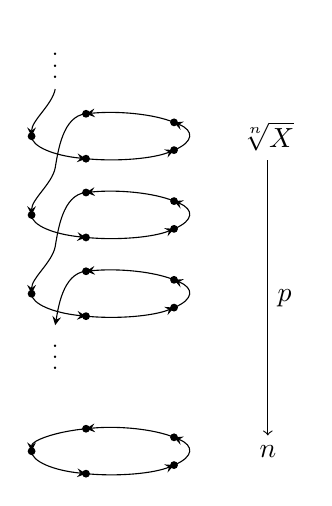
\begin{tikzpicture}
    \node (A) at (2,2) {$\sqrt[n]X$};
    \node (B) at (2,-2) {$\bn{n}$};
    \draw[->] (A) -- node[auto] {$p$} (B);
    \foreach \y in {-2,0,1,2}
    { \begin{scope}[shift={(0,\y)}]
        \foreach \x in {0,...,4}
        { \node[fill,circle,inner sep=1pt] at (180+72*\x:1 and .3) {}; }
        \foreach \x in {0,...,3}
        { \draw[-stealth] (180+72*\x:1 and .3) arc(180+72*\x:252+72*\x:1 and .3); }
      \end{scope} }
    \begin{scope}[shift={(0,-2)}]
      \draw[-stealth] (108:1 and .3) arc(108:180:1 and .3);
    \end{scope}
    \foreach \y in {1,2}
    { \begin{scope}[shift={(0,\y)}]
        \draw[-stealth] (108:1 and .3)
        .. controls ++( 5:-.3) and ++(80:.2) .. (-.7,-.4)
        .. controls ++(80:-.2) and ++(90:.2) .. (-1,-1);
      \end{scope} }
    \draw[-stealth] (108:1 and .3)
    .. controls ++( 5:-.3) and ++(80:.2) .. (-.7,-.4);
    \node (dz) at (-.7,-.7) {\footnotesize $\vdots$};
    \begin{scope}[shift={(0,3)}]
      \draw[-stealth] (-.7,-.4)
      .. controls ++(80:-.2) and ++(90:.2) .. (-1,-1);
    \node (da) at (-.7,0) {\footnotesize $\vdots$};
    \end{scope}
  \end{tikzpicture}
  \caption{The $n$'th root of an endomorphism, with projection}
  \label{fig:rootproj}
\end{figure}

